\section{Resultados}

\begin{frame}{El frente de Pareto}
    \begin{columns}[c]
        \begin{column}{0.55\textwidth}
            \centering
            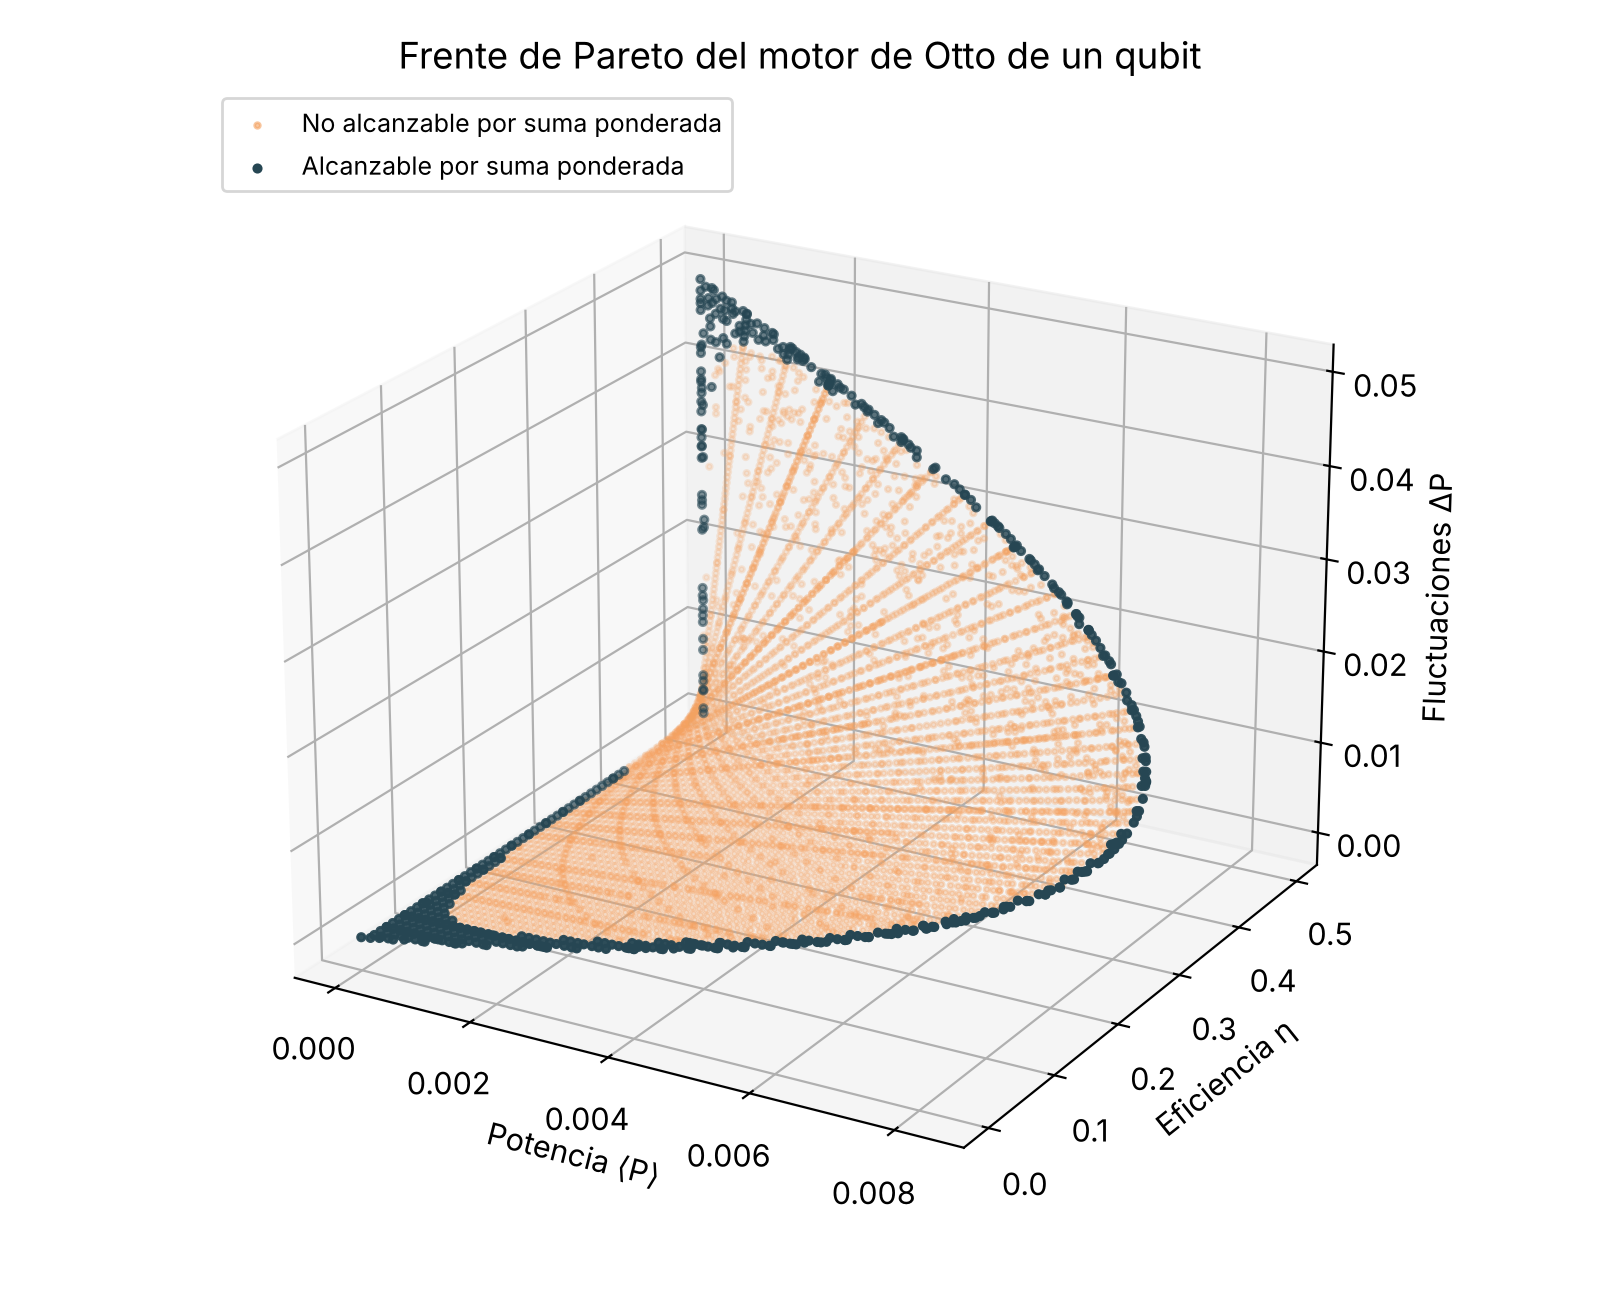
\includegraphics[height=0.78\textheight]{fig1_frente_3d.png}
        \end{column}
        \begin{column}{0.42\textwidth}
            \begin{itemize}
                \setlength{\itemsep}{8pt}
                \item A $\eta$ fija: una \textbf{recta}.
                \item La superficie es una \textbf{silla}.
                \item Naranja: inalcanzable con suma ponderada.
            \end{itemize}
        \end{column}
    \end{columns}
\end{frame}

\begin{frame}{Potencia contra eficiencia}
    \begin{columns}[c]
        \begin{column}{0.60\textwidth}
            \centering
            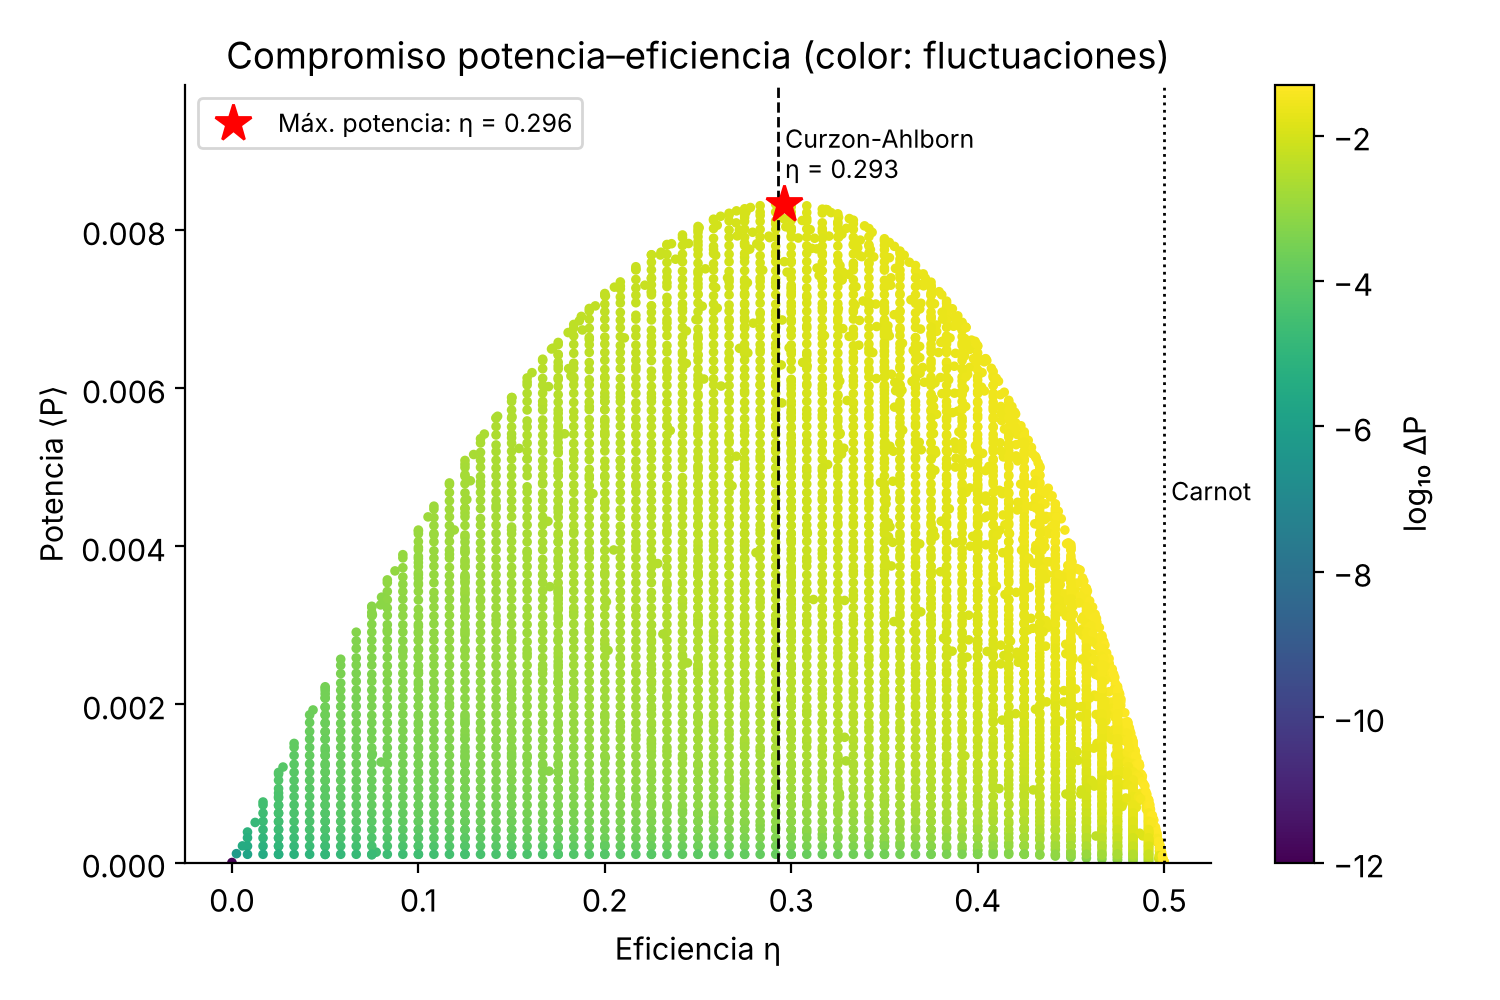
\includegraphics[height=0.75\textheight]{fig2_potencia_eficiencia.png}
        \end{column}
        \begin{column}{0.38\textwidth}
            Máxima potencia:
            \[ \eta^* = 0{,}296 \]
            Curzon--Ahlborn:
            \[ \eta_{CA} = 1 - \sqrt{T_c/T_h} = 0{,}293 \]
            Carnot ($0{,}5$): potencia cero.
        \end{column}
    \end{columns}
\end{frame}

\begin{frame}{El frente sigue la relación de incertidumbre}
    \begin{columns}[c]
        \begin{column}{0.55\textwidth}
            \centering
            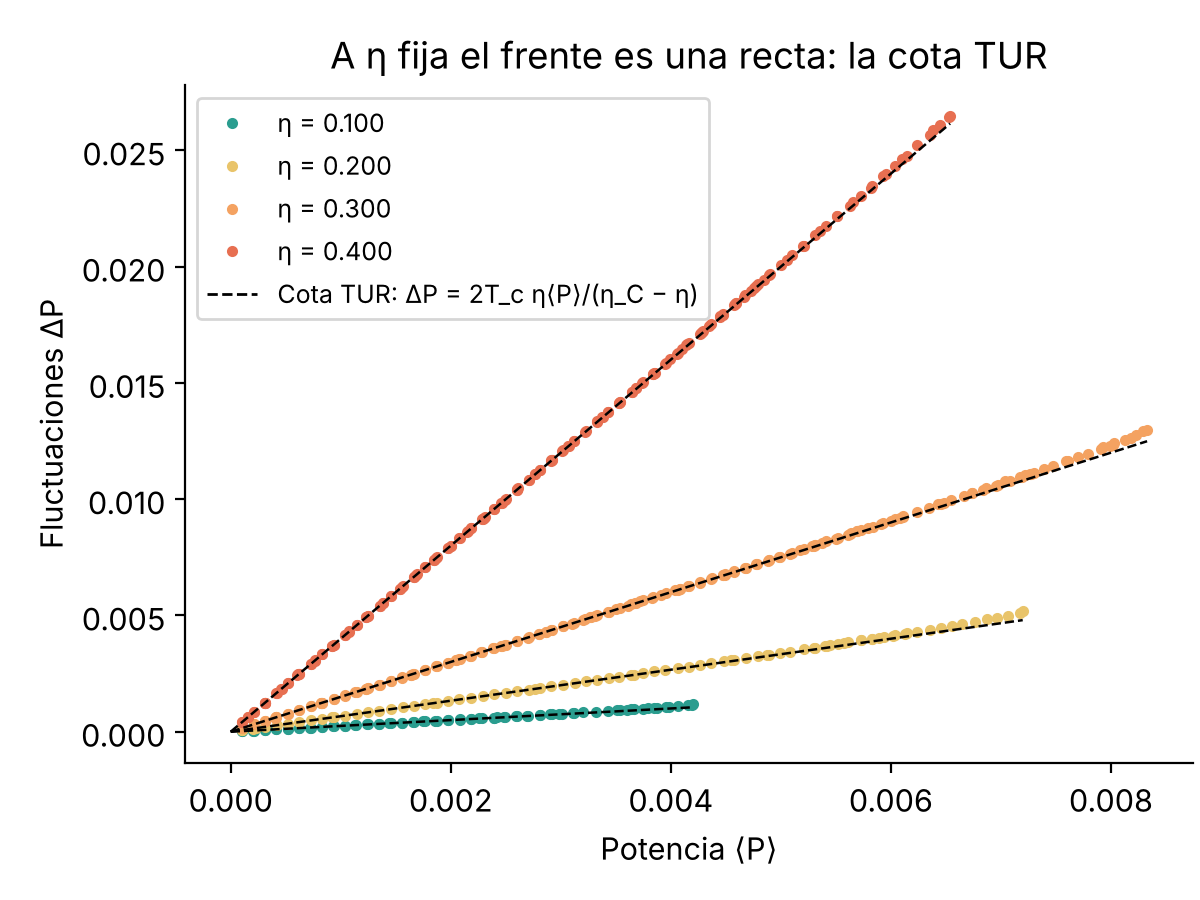
\includegraphics[height=0.72\textheight]{fig5a_tur_rectas.png}
        \end{column}
        \begin{column}{0.42\textwidth}
            En el frente:
            \[
                \dP \;\approx\; \frac{2T_c\,\eta}{\eta_C - \eta}\,\avg{P}
            \]
            \begin{itemize}
                \item mediana $\xi = 0{,}998$
                \item máximo $\xi = 1{,}0056$ (motor cíclico)
            \end{itemize}
        \end{column}
    \end{columns}
\end{frame}

\begin{frame}{¿Qué algoritmo encuentra mejor el frente?}
    \centering
    {\large
    \begin{tabular}{lcc}
        \toprule
        Algoritmo & HV ($\uparrow$) & IGD$^+$ ($\downarrow$) \\
        \midrule
        \textbf{MOEA/D-AWA} & $\mathbf{1{,}0407}$ & $\mathbf{0{,}0202}$ \\
        MOEA/D & $1{,}0385$ & $0{,}0258$ \\
        NSGA-III & $1{,}0315$ & $0{,}0252$ \\
        NSGA-II & $1{,}0065$ & $0{,}0424$ \\
        Suma ponderada & $0{,}9668$ & $0{,}0748$ \\
        \midrule
        Frente de referencia & $1{,}0801$ & $0$ \\
        \bottomrule
    \end{tabular}
    }

    \vspace{14pt}
    MOEA/D-AWA gana en ambas métricas; NSGA-II deja huecos con 3 objetivos.

    \vspace{4pt}
    {\small Medias sobre 10 semillas, normalizadas por el frente de referencia.}
\end{frame}

\begin{frame}{¿Por qué no basta una suma ponderada?}
    \begin{columns}[c]
        \begin{column}{0.50\textwidth}
            \centering
            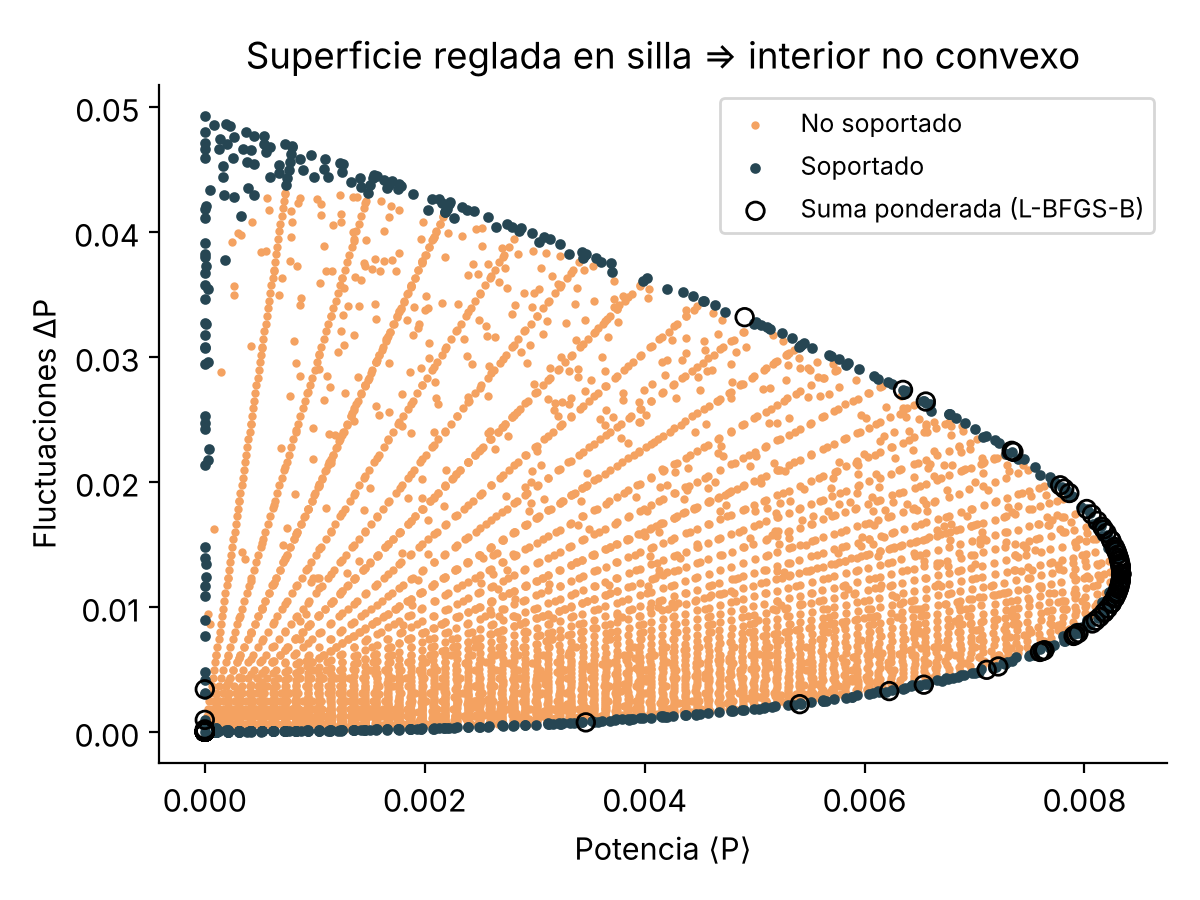
\includegraphics[height=0.72\textheight]{fig5b_soportados.png}
        \end{column}
        \begin{column}{0.47\textwidth}
            \begin{tabular}{lc}
                \toprule
                Objetivos & inalcanzable \\
                \midrule
                $(\avg{P}, \eta, \dP)$ & $90\%$ \\
                $(\avg{P}, \dP, \Sigma)$ & $13\%$ \\
                \bottomrule
            \end{tabular}

            \vspace{8pt}
            Con $\eta$: silla. Con $\Sigma$: convexa.

            \vspace{4pt}
            Aun así la suma ponderada pierde 6--7\% de HV: sus soluciones quedan amontonadas.

            \vspace{8pt}
            \textbf{AWA corrige ambos problemas.}
        \end{column}
    \end{columns}
\end{frame}
